%%% PREAMBLE - Do not touch %%%%%%%%%%%%%%%%%%%%%%%%%%%%%%%%%%%%%%%%%%%%%%%%%%%%%%
\documentclass[10pt,twocolumn,letterpaper]{article}
\usepackage[utf8]{inputenc}
\usepackage[portuges,brazil,english]{babel}
%\usepackage{model}
\usepackage{times}
\usepackage{epsfig}
\usepackage{graphicx}
\usepackage{amsmath}
\usepackage{amssymb}
\usepackage{color}
\usepackage[pagebackref=true,breaklinks=true,letterpaper=true,colorlinks,bookmarks=false]{hyperref}
\usepackage{numberedblock}
\usepackage{cleveref}
%\input{pics/abaco}

%\cvprfinalcopy % *** Uncomment this line for the final submission
\def\httilde{\mbox{\tt\raisebox{-.5ex}{\symbol{126}}}}
%\ifcvprfinal\pagestyle{empty}\fi

\newcommand{\TODO}[1]{TODO: #1}
\newcommand{\CITEONE}[2]{\mbox{#1 \cite{#2}}}
\newcommand{\CITETWO}[3]{\mbox{#1 and #2 \cite{#3}}}
\newcommand{\CITEN}[2]{\mbox{#1 et al. \cite{#2}}}

\addto\captionsenglish{%
  \renewcommand{\figurename}{Fig.}%
  \renewcommand{\refname}{Referências}%
}

%%% Report beginning %%%%%%%%%%%%%%%%%%%%%%%%%%%%%%%%%%%%%%%%%%%%%%%%%%%%%%%%%%%%%%
\begin{document}

%%% Title and authors %%%%%%%%%%%%%%%%%%%%%%%%%%%%%%%%%%%%%%%%%%%%%%%%%%%%%%%%%%%%
\title{Relatório Trabalho 3}
\author{Raphael Adamski \\227179}

%%% Abstract %%%%%%%%%%%%%%%%%%%%%%%%%%%%%%%%%%%%%%%%%%%%%%%%%%%%%%%%%%%%%%%%%%%%%
\maketitle
%\begin{abstract}
Este relatório é parte de uma série de trabalhos da disciplina \emph{MO443 - Introdução ao Processamento de Imagem Digital} lecionada pelo Professor Hélio Pedrini na Universidade Estadual de Campinas no primeiro semestre de 2018.
%\end{abstract}

%%% Introduction %%%%%%%%%%%%%%%%%%%%%%%%%%%%%%%%%%%%%%%%%%%%%%%%%%%%%%%%%%%%%%%%%
\section{Ambiente}
O algoritmo desenvolvido necessita de um ambiente com Python 3.x instalado, além das bibliotecas \emph{OpenCV}\footnote{\url{https://opencv.org/}}, \emph{Numpy}\footnote{\url{http://www.numpy.org/}}, \emph{imutils}, \emph{PIL} e \emph{Pytesseract}. Este ultimo é apenas uma interface para um comando do sistema operacional (SO), por isso deve estar instalado no SO a biblioteca \emph{Tesseract Open Source OCR Engine }\footnote{https://github.com/tesseract-ocr/tesseract}.

%%% Add section %%%%%%%%%%%%%%%%%%%%%%%%%%%%%%%%%%%%%%%%%%%%%%%%%%%%%%%%%%%%%%%%%%
\section{Algoritmo}

Dado o ambiente como esperado, basta rodar o código fornecido como seguinte uso:\\
\begin{numVblock}
alinhar.py [-h] -i INPUT [-o OUTPUT]
[-m {projection,hough}]
[-p {crop,sobel,otsu,contours,gray}]
[-c CROP]
\end{numVblock}
em quem o argumento \texttt{-i} é o endereço da imagem de entrada para ser encontrado o texto e alinhada, \texttt{-o} é o endereço para salvar a imagem de saída, \texttt{-m} é a técnica a ser utilizada para encontrar o ângulo de rotação da imagem (Hough ou Projeção Horaizontal), \texttt{-p} são os métodos de pré-processamento a serem utilizados (permitindo uma combinação de vários entre filtro de Sobel, Otsu Threshold, recortar, encontrar contornos) e \texttt{-c} é parâmetro para definir o tamanho da janela do recorte, caso selecionado no pré-processamento.(\emph{crop}). Utilizando \texttt{-h} mostra-se o uso e descrição do programa.\\
\subsection{Pré-processamento}
No código foram implementadas quatro técnicas para esta etapa. Vale ressaltar que independentemente dos parâmetros de \texttt{-p} passados, sempre será feito uma conversão para escala de cinza (parâmetro \texttt{gray}), já que ambos algoritmos para encontrar o ângulo esperam imagens com uma dimensão de profundidade.\\
\begin{figure}
    \centering
    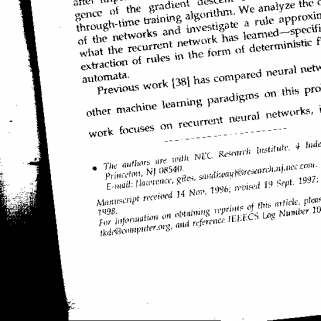
\includegraphics[scale=0.5]{sample3.png}
    \caption{Imagem de exemplo com bordas pretas fora da imagem.\label{fig:sample3}}
\end{figure}
As técnicas estão ordenadas na ordem em que são aplicadas:
\subsubsection*{Recorte}
O parâmetro \texttt{crop} quando usado permite recortar a imagem com uma janela de 500 pixels por padrão, localizada no centro da imagem. O tamanho da janela é configurável por \texttt{-c} seguido de um número inteiro.
\subsubsection*{Filtro Sobel}
Este filtro detector de bordas é usado quando é passado \texttt{sobel} na linha de execução do programa. Basicamente ele realça bordas usando gradiente da imagem. A função utilizada esta presente na biblioteca \emph{OpenCV}. Na Figura \ref{fig:sobel} é possível visualizar o efeito da técnica.
\begin{figure}
    \centering
    \includegraphics[scale=0.6]{sobel.png}
    \caption{Aplicação do filtro de Sobel na Figura \ref{fig:sample3}.\label{fig:sobel}}
\end{figure}
\subsubsection*{Otsu Threshold}
Esta é uma técnica de binarização local da imagem, já implementada em \emph{OpenCV} e é ativada usando parâmetro \texttt{otsu}. É possível ver seu efeito na Figura \ref{fig:otsu}.
\begin{figure}
    \centering
    \includegraphics[scale=0.6]{binary.png}
    \caption{Aplicação do Otsu threshold na Figura \ref{fig:sample3}.\label{fig:otsu}}
\end{figure}
\subsubsection*{Reconhecimento de Contornos}
Usando \texttt{contours} é possível melhorar o processamento identificando previamente formas, como imagens e tabelas (vide \ref{fig:com_figura} e \ref{fig:sem_figura}). As mesmas são tiradas quando reconhecidas pela função \texttt{cv2.findContours} que implementa a técnica proposta por \cite{Suzuki85}.\\
\begin{figure}
    \centering
    \includegraphics[scale=0.4]{wimage.png}
    \caption{Imagem com figuras com Otsu Threshold.\label{fig:com_figura}}
\end{figure}
\begin{figure}
    \centering
    \includegraphics[scale=0.4]{woimage.png}
    \caption{Aplicação da remoção de contornos na Figura \ref{fig:com_figura}.\label{fig:sem_figura}}
\end{figure}
Quando a imagem esta deslocada e com bordas pretas, é possível também reconhecer o formato da folha e retirar este fundo preto que poderia interferir no processamento. Como é possível ver comparando a Figura \ref{fig:sample3} e \ref{fig:contours}.\\
\begin{figure}
    \centering
    \includegraphics[scale=0.6]{contours.png}
    \caption{Aplicação da remoção de contornos na Figura \ref{fig:sample3}.\label{fig:contours}}
\end{figure}

\subsection{Detecção do Ângulo}
Como é perceptível nas Figuras \ref{fig:otsu} e \ref{fig:com_figura} , as imagens que passaram por binarização usando Otsu ou Sobel ficaram com o fundo preto, isso foi feito de maneria proposital pois ambos os métodos explicados a seguir funcionam mais adequadamente com pixels relevantes (neste caso letras) tendo valor, que neste caso seria 255 e cor branca.
\subsubsection*{Projeção Horizontal}
A técnica se baseia em rotacionar a imagem em 180 graus (pois não é possível prever se o texto esta invertido) e para cada ângulo calcular a soma dos pixels em cada linha, por isso a imagem com representatividade apenas nas letras ( fundo preto, letras brancas). O ângulo com  a linha que somasse maior valor é escolhido como ângulo de correção da imagem.\\
Como é perceptível, fundo com cor igual das letras, como na Figura \ref{fig:sample3}, e imagens tornam esse algoritmo muito suscetível a falhas. Além disso, a função utilizada para rotação (\texttt{imutils.rotate\_bound}) preenche o fundo da imagem com preto, sendo este outro motivo para inverter a cor das letras e o fundo.\\
\subsubsection*{Transformada de Hough}
Esta transformada leva os pontos com intensidade maior que 10, na escala de 0 a 255, para outro plano discretizado por $\rho = x\times cos(\theta) + y\times sen(\theta)$. Usando o valor de $\theta$ da tabela do ponto que obtiver maior número de curvas cruzando, indicará o ângulo de inclinação do texto.\\
Este método é altamente suscetível a falhas com fundos com cor, como na Figura \ref{fig:sample3}, pois todos os pontos claros (maior que 10) serão transformados para o plano de Hough e irão influenciar na escolha do ângulo. A Figura \ref{fig:hough_orig} mostra uma faixa amarela escura que representa a influencia errada do fundo da imagem, e que consequentemente leva a escolha errada do ângulo. Já na Figura \ref{fig:hough_contours} vemos claramente que o angulo de aproximadamente 84 graus esta acumulando vários pequenos pontos amarelos, com alta concentração de curvas cruzando, sendo assim a melhor escolha.
\begin{figure}
    \centering
    \includegraphics[scale=0.6]{hough_orig.png}
    \caption{Transformada de Hough dos pixels da Figura \ref{fig:otsu} (sem remoção do fundo).\label{fig:hough_orig}}
\end{figure}
\begin{figure}
    \centering
    \includegraphics[scale=0.6]{hough_contours.png}
    \caption{Transformada de Hough dos pixels da Figura \ref{fig:contours} (com remoção do fundo).\label{fig:hough_contours}}
\end{figure}
\subsection{Detecção do Texto}
É aplicado a técnica de \emph{Optical Character Recognition} (OCR) antes e depois da rotação para mostrar casos em que houve melhoria. A função utilizada da do pacote citado foi  \texttt{pytesseract.image\_to\_string}.

%%% Add section %%%%%%%%%%%%%%%%%%%%%%%%%%%%%%%%%%%%%%%%%%%%%%%%%%%%%%%%%%%%%%%%%%
\section{Saída}
Durante a execução é mostrado a imagem original ao usuário em uma janela, e em seguida as imagens de cada processo de pré-processamento selecionado.
Por fim a imagem original é rotacionada negativamente com o ângulo de inclinação encontrado.
O console mostra o texto antes e depois da rotação além do ângulo de rotação para melhorar a imagem.\\
A imagem rotacionada é salva caso na execução tenha sido passado o argumento \texttt{-o} com o caminho para o arquivo.

%%% Add section %%%%%%%%%%%%%%%%%%%%%%%%%%%%%%%%%%%%%%%%%%%%%%%%%%%%%%%%%%%%%%%%%%
\section{Testes}
Os testes mostraram que ambas as técnicas de reconhecimento da inclinação têm os mesmos resultados, contudo a Transformada de Hough implementado pelo autor precisa ser otimizada, pois o tempo de execução é muito maior que a projeção horizontal.\\
Apenas o uso de binarização (Otsu ou Sobel) foi bem eficaz em imagens com fundo sólido. Porém em testes com imagens de pior qualidade ou estruturas que não fossem apenas texto, como Figura \ref{fig:sample3} e \ref{fig:com_figura}, o desempenho dos algoritmos ficava distante do ideal.\\
Aplicando recortes no centro da imagem em alguns casos ajudou a evitar bordas com problemas, contudo caso o recorte concentrasse em uma imagem, como a Figura \ref{fig:com_figura}, existia ainda uma dificuldade para processamento.\\
Então aplicando a técnica da reconhecimento de contorno foi possível obter sucesso nas imagens de teste usando filtro de Sobel e projeção horizontal.

%%% Add section %%%%%%%%%%%%%%%%%%%%%%%%%%%%%%%%%%%%%%%%%%%%%%%%%%%%%%%%%%%%%%%%%%
\section{Condições não tratadas}
Além de não serem tratados os casos em que o ambiente não está estabelecido como descrito acima, vale ressaltar que não se verifica se o endereço da imagem passado como parâmetro é válido, o que pode resultar em erros de execução devido a objetos vazios.\\
A pasta do local de saída da imagem gerada pelo algoritmo de codificação deve existir, caso contrário a mesma não é salva.\\

%%% Add section %%%%%%%%%%%%%%%%%%%%%%%%%%%%%%%%%%%%%%%%%%%%%%%%%%%%%%%%%%%%%%%%%%
\section{Condições tratadas}
Imagens podem ser coloridas ou em escala de cinza e de diferentes extensões, já que a biblioteca trata a maioria dos formatos\footnote{\url{https://docs.opencv.org/2.4/modules/highgui/doc/reading_and_writing_images_and_video.html}}. O arquivo de saída não precisa existir, pois é criado caso não exista, com a extensão \emph{.png}. Se existir e tiver algum conteúdo, o mesmo é apagado.

%%% Add section %%%%%%%%%%%%%%%%%%%%%%%%%%%%%%%%%%%%%%%%%%%%%%%%%%%%%%%%%%%%%%%%%%
\section{Considerações finais}
O arquivo entregue contem um diretório \emph{.git} em que é possível verificar a evolução do código pelos \emph{commits\footnote{\url{https://git-scm.com/docs/gittutorial/2.2.0}}}.
Também existem imagens para teste oriundas de \url{https://www.ic.unicamp.br/~helio/imagens_inclinadas_png/}.

%%% References %%%%%%%%%%%%%%%%%%%%%%%%%%%%%%%%%%%%%%%%%%%%%%%%%%%%%%%%%%%%%%%%%%%

\begin{thebibliography}{1}

\bibitem{Suzuki85}
Suzuki, S. and Abe, K.,
\newblock Topological Structural Analysis of Digitized Binary Images by Border Following.
\newblock CVGIP 30 1,
\newblock pp 32-46 (1985)

\end{thebibliography}

\end{document}
